\documentclass[12pt, final]{CSP}
\usepackage{amssymb}
\usepackage{changepage}
\usepackage[margin=3.5cm]{geometry}
\usepackage{graphicx}
\usepackage{amssymb,amsmath,amsfonts,eurosym,geometry,ulem,graphicx,caption,color,sectsty,comment,footmisc,caption,natbib,pdflscape,subfigure,array,hyperref}
\begin{document}

\begin{frontmatter}

\title{Replication of Import Competition and Internal Migration}

\author[mymainaddress]{Chuxin Liu}

\address[mymainaddress]{CUNY Graduate Center}

\begin{abstract}\rm
\begin{adjustwidth}{2cm}{2cm}{\itshape\textbf{Abstract:}} 
This paper replicates the main result of "Import Competition and Internal Migration"\cite{greenland2019import}, authored by Andrew Greenland, John Lopresti, and Peter McHenry and published on \textit{Review of Economics and Statistics} in 2019. The replication result is very close to the original work while slight downward estimates are observed. This paper also has an extension which commuting zone size is taken into account. It is shown that for larger cities, the negative effect of import competition on population growth will be smaller. 
\newline 
\newline 
\newline 
\end{adjustwidth}
\end{abstract}
\end{frontmatter}

\section{Introduction}
\label{}
\noindent
This paper replicates the main result of "Import Competition and Internal Migration"\cite{greenland2019import}, authored by Greenland, Andrew, John Lopresti, and Peter McHenry and published on \textit{Review of Economics and Statistics} in 2019. The replication result is very close to the original work while slight downward estimates are observed. This paper also has an extension which commuting zone size is taken into account. It is shown that for larger cities, the negative effect of import competition on population growth will be smaller. 
\newline
\newline
Greenland et al (2019)\cite{greenland2019import} examine the U.S. internal migration response to increased import competition following the granting of Permanent Normal Trade Relations to China in 2011. Using a variety of data sets and empirical approaches, they find that local labor markets most exposed to the policy change experienced a relative reduction in population growth over the following decade.
\newline
\newline
This paper is part of the big economic question of winners and losers in trade. While the gains from trade is spread throughout the economy, costs of trade is highly concentrated. More specifically, the cost is concentrated among low education and low wage labor force. In the literature, there is documented evidence that trade shock leads to lower wages, lower labor force participation, and higher unemployment among low education and low wage population. It is also found that they experience worse physical health, worse mental health, and increased mortality risk. Also, the cost is concentrated geographically. Literature documents that areas with high trade shock also experienced losses in income, lower tax base and less funding for public good. Therefore, there is huge challenge for both trade policy making and place-based policy making.  
\newline
\newline
It is worth noting that when this paper was written, no documented migration due to trade shock. Therefore, this paper is the first in the literature to address how people adjust to changing labor market opportunities by moving. After this paper was written, there are some PhD students working on similar topic, which also tries to address how labor move across space in react to trade shock and technology shock. I have heard two presentations from the Urban Economics Summer School, but I have not found the citation of those two papers. 
\newline
\newline
The major data used in this paper is US Census, NELS:88 and ELS:2002, and IRS Migration Data. While NELS and ELS help address childhood to adult location transition and IRS Migration Data addresses timeline of population change in react to trade shock, the US Census produces the most important results of this paper. It is representative of the whole country, and it is sourced from administrative data, which confirms the reliability of the data used in the research. Ideally, we might want to have more years as US Census is only done in every 10 years. 
\newline
\newline
The research is done with empirical approach without theoretical framework, but it is convincing since the aim is only to document migration, without the need to estimate migration cost, trade cost, trade loss etc. In terms of internal validity, this paper’s key independent variable of interest is constructed by previous work. The authors fully take advantage of the previous work done by famous economists, including David Autor, Pierce and Schott, which allows minimal discussion on endogeneity. In my opinion, the paper is very convincing. 
\newline
\newline
The remainder of the paper proceeds as follows. Section 2 shows the replication by describing data sets I use and showing the results I have. In section 3, I will discuss the difference between replication and the original paper. I will compare the data I generated and the data from published replication package. In section 4, I will conduct an extension by taking commuting zone size into account and show that larger commuting zones experience less population loss while holding trade shock constant. Section 5 includes a brief discussion and conclusion.


\section{Replication}
\noindent
\subsection{Data}
To replicate the main result of this paper, the following data sets are used.
\begin{itemize}
\item \textbf{US Census} 
\newline
\newline
The US Census is representative of the whole country, available every 10 years on IPUMS. It is a well-known data source and provides reliable population measures. From IPUMS, location is coded as “county” or “puma”. In order to use them in this paper, “county” or “puma” will be converted into commuting zones using crosswalk files.
\newline
\item \textbf{Trade shock measure by Pierce and Schott (2016)} \cite{pierce2016surprisingly} 
\newline
\newline
Pierce and Schott (2016) \cite{pierce2016surprisingly} find that import competition for United State industries changed dramatically when the U.S. granted Permanent Normal Trade Relations (PNTR) to China in 2001. Pierce and Schott (2016) \cite{pierce2016surprisingly} take a difference-in-differences approach to examine the effects of the policy change, exploiting the variation in the potential tariff increase across industries before and after the granting of PNTR in 2001. In addition to increased import competition, they show that the industries most exposed to the policy change experienced a reduction in employment in the years after 2001. They define the difference between the observed NTR tariff rates and the potential non-NTR rates in industry j as the “NTR gap” facing the industry. As the outcome of interest is inherently geographical, this paper requires a geographically based measure of import competition. To obtain this, the paper create a commuting zone (henceforth CZ) level measure of the NTR gap. CZs, a concept pioneered by Tolbert and Sizer (1996)\cite{tolbert1996us} and employed recently in a trade context by Autor et al. (2016)\cite{autor2016china}, are approximations of local labor markets, created using journey-to-work data such that individuals living in a given CZ are highly likely to work in the same CZ. There are 722 CZs in this data, spanning the entire continental United States. Hawaii and Alaska are not included. This paper creates a CZ-level measure of the NTR gap by weighting industry NTR gaps by the share of employment in CZ c accounted for by each industry j.
\newline
\newline
    \begin{equation}
        NTR\: \: Gap_j=Non\: \:NTR\: \: Tariff_j - NTR\: \: Tariff_j
    \end{equation}
    \begin{equation}
        NTR\: \: Gap_c=\sum_{j} \frac{L_{cj}}{L_c}*NTR\: \: Gap_j
\end{equation}
\newline
\item \textbf{PUMA to CZ crosswalk by Peter McHenry}
\newline
\newline
While I was exploring ways to convert “county” or “puma” into commuting zones, I noticed that one of the authors of the paper, Peter McHenry, posted crosswalk files on his personal websites. These files are directly used in converting location units for my replication.
\newline
\end{itemize}

\begin{figure}[h]
\caption{Histogram of Trade Shock}
\centering
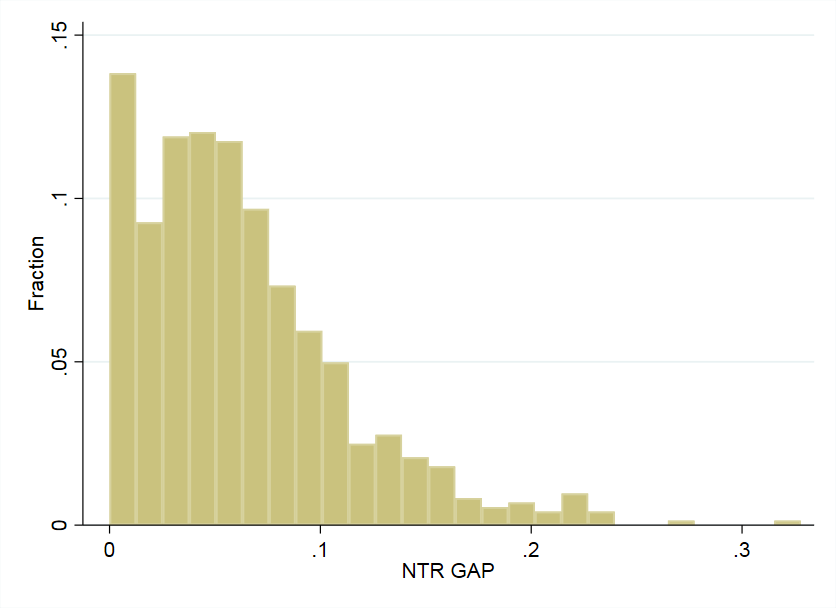
\includegraphics[width=0.8\textwidth]{Figure_A1.png}
\end{figure}

\subsection{Result}
Firstly, I replicate the main figures of the paper. Figure 1 is the histogram of NTR Gap, which is the key independent variable of this paper: the measure of trade shock. Figure 1 is successfully replicated. 
\newline
\newline
Figure 2 panel d is the map of NTR Gap, which is also successfully replicated. I extend the map by adding population change pre shock (panel a), population change post shock (panel b), and the difference of post and pre shock (panel c) to show spatial correlation. As it is shown, that places that are darker in panel (d), where places experienced larger import competition, are also the places that are lighter in panel (c), where population growth is lower. 
\newline
\newline
\begin{figure}[h]
\caption{Geography of Population Change and Trade Shock}
\centering
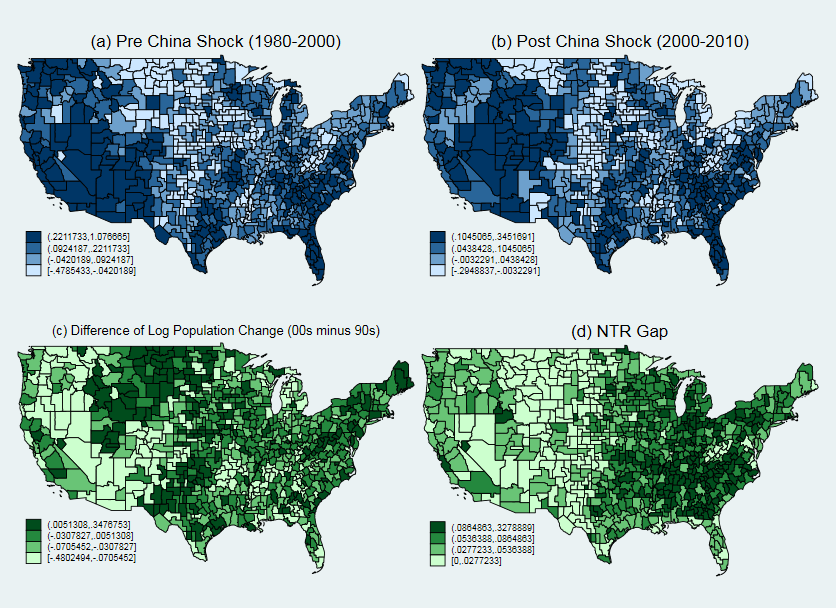
\includegraphics[width=1\textwidth]{popNTR}
\end{figure}
\newline
\newline
I go on to replicate the important tables in the paper. Firstly, Table 1 and Table 2 replicate that first table in the original paper, which regress ten-year changes in Log CZ Population on import competition. Different specifications across columns are due to different levels of controls and 2 age groups: 15-64 and 15-34. I am able to obtain very similar estimate and significance, while my replication estimates are slightly smaller and slightly less significant. The $R^2$ in my replication is around 0.03 less than the original paper too. Overall, the replication is reasonable. 
\newline
\newline

\begin{table}[htbp]\centering
\def\sym#1{\ifmmode^{#1}\else\(^{#1}\)\fi}
\caption{Import Competition and 10-year Changes in Log CZ Population (aged 15-34), Census}
\begin{tabular}{l*{4}{c}}
\hline
\hline 
\toprule
                    &\multicolumn{1}{c}{(1)}&\multicolumn{1}{c}{(2)}&\multicolumn{1}{c}{(3)}&\multicolumn{1}{c}{(4)}\\
                    &\multicolumn{1}{c}{$\Delta ln(pop_{15-64})$}&\multicolumn{1}{c}{}&\multicolumn{1}{c}{}&\multicolumn{1}{c}{}\\
\hline
\midrule
NTR Gap             &   -0.186*  &   -0.251***&   -0.190   &   -0.186   \\
                    &  (0.098)   &  (0.081)   &  (0.143)   &  (0.135)   \\
\addlinespace
Lag 15-64 Change    &    0.552***&    0.545***&    0.524***&    0.519***\\
                    &  (0.037)   &  (0.034)   &  (0.035)   &  (0.037)   \\
\addlinespace
Hispanic Share      &            &    0.083*  &    0.067   &    0.062   \\
                    &            &  (0.046)   &  (0.047)   &  (0.051)   \\
\addlinespace
Under 25 Share      &            &    0.336***&    0.412***&    0.422***\\
                    &            &  (0.114)   &  (0.118)   &  (0.125)   \\
\addlinespace
Black Share         &            &   -0.117*  &   -0.150***&   -0.156***\\
                    &            &  (0.067)   &  (0.054)   &  (0.050)   \\
\addlinespace
American Indian Share&            &   -0.206***&   -0.108*  &   -0.113*  \\
                    &            &  (0.056)   &  (0.064)   &  (0.064)   \\
\addlinespace
Asian Share         &            &    0.058   &   -0.484***&   -0.479***\\
                    &            &  (0.237)   &  (0.174)   &  (0.169)   \\
\addlinespace
Neighbor CZ Effect  &            &            &    0.083   &    0.254   \\
                    &            &            &  (0.305)   &  (0.288)   \\
\addlinespace
Routineness         &            &            &    0.004** &    0.003*  \\
                    &            &            &  (0.002)   &  (0.002)   \\
\addlinespace
Offshorability      &            &            &    0.015   &    0.017   \\
                    &            &            &  (0.013)   &  (0.014)   \\
\addlinespace
Capital-Labor Ratio &            &            &    0.000   &    0.001   \\
                    &            &            &  (0.013)   &  (0.014)   \\
\addlinespace
Skill Intensity     &            &            &    0.096   &    0.104*  \\
                    &            &            &  (0.059)   &  (0.060)   \\
\addlinespace
Female Labor Force Share&            &            &   -0.374   &   -0.392   \\
                    &            &            &  (0.293)   &  (0.339)   \\
\addlinespace
College Educated Share&            &            &    0.001   &    0.001   \\
                    &            &            &  (0.001)   &  (0.001)   \\
\addlinespace
Debt to Income      &            &            &            &    0.018   \\
                    &            &            &            &  (0.031)   \\
\addlinespace
HPI Break           &            &            &            &    0.144** \\
                    &            &            &            &  (0.062)   \\
\midrule
Observations        &     1444   &     1444   &     1444   &     1322   \\
\(R^{2}\)           &    0.678   &    0.693   &    0.708   &    0.711   \\
Region-Year FE      &        Y   &        Y   &        Y   &        Y   \\
\hline
\bottomrule
\multicolumn{5}{l}{\footnotesize Standard errors in parentheses}\\
\multicolumn{5}{l}{\footnotesize $* p<.1, ** p<0.05, *** p<0.01$}\\
\end{tabular}
\end{table}

\newline
\newline

\begin{table}[htbp]\centering
\def\sym#1{\ifmmode^{#1}\else\(^{#1}\)\fi}
\caption{Import Competition and 10-year Changes in Log CZ Population (aged 15-34), Census}
\begin{tabular}{l*{4}{c}}
\hline
\hline 
\toprule
                    &\multicolumn{1}{c}{(1)}&\multicolumn{1}{c}{(2)}&\multicolumn{1}{c}{(3)}&\multicolumn{1}{c}{(4)}\\
                    &\multicolumn{1}{c}{$\Delta ln(pop_{15-34})$}&\multicolumn{1}{c}{}&\multicolumn{1}{c}{}&\multicolumn{1}{c}{}\\
\hline
\midrule
NTR Gap             &   -0.580***&   -0.682***&   -0.421** &   -0.399** \\
                    &  (0.126)   &  (0.107)   &  (0.193)   &  (0.185)   \\
\addlinespace
Lag 15-34 Change    &    0.353***&    0.344***&    0.331***&    0.323***\\
                    &  (0.046)   &  (0.044)   &  (0.047)   &  (0.047)   \\
\addlinespace
Hispanic Share      &            &    0.087   &    0.081   &    0.068   \\
                    &            &  (0.056)   &  (0.062)   &  (0.064)   \\
\addlinespace
Under 25 Share      &            &    0.261*  &    0.397** &    0.425** \\
                    &            &  (0.155)   &  (0.172)   &  (0.172)   \\
\addlinespace
Black Share         &            &   -0.157** &   -0.171***&   -0.181***\\
                    &            &  (0.080)   &  (0.065)   &  (0.062)   \\
\addlinespace
American Indian Share&            &   -0.189** &   -0.089   &   -0.084   \\
                    &            &  (0.086)   &  (0.095)   &  (0.091)   \\
\addlinespace
Asian Share         &            &   -0.228   &   -0.827***&   -0.782***\\
                    &            &  (0.307)   &  (0.243)   &  (0.238)   \\
\addlinespace
Neighbor CZ Effect  &            &            &   -0.319   &   -0.087   \\
                    &            &            &  (0.422)   &  (0.388)   \\
\addlinespace
Routineness         &            &            &    0.003   &    0.002   \\
                    &            &            &  (0.002)   &  (0.002)   \\
\addlinespace
Offshorability      &            &            &    0.001   &    0.006   \\
                    &            &            &  (0.019)   &  (0.020)   \\
\addlinespace
Capital-Labor Ratio &            &            &   -0.007   &   -0.007   \\
                    &            &            &  (0.017)   &  (0.018)   \\
\addlinespace
Skill Intensity     &            &            &    0.169** &    0.178** \\
                    &            &            &  (0.086)   &  (0.089)   \\
\addlinespace
Female Labor Force Share&            &            &   -0.099   &   -0.117   \\
                    &            &            &  (0.399)   &  (0.444)   \\
\addlinespace
College Educated Share&            &            &    0.002   &    0.002   \\
                    &            &            &  (0.001)   &  (0.001)   \\
\addlinespace
Debt to Income      &            &            &            &    0.052   \\
                    &            &            &            &  (0.035)   \\
\addlinespace
HPI Break           &            &            &            &    0.224** \\
                    &            &            &            &  (0.088)   \\
\midrule
Observations        &     1444   &     1444   &     1444   &     1322   \\
\(R^{2}\)           &    0.607   &    0.619   &    0.634   &    0.641   \\
Region-Year FE      &        Y   &        Y   &        Y   &        Y   \\
\hline
\bottomrule
\multicolumn{5}{l}{\footnotesize Standard errors in parentheses}\\
\multicolumn{5}{l}{\footnotesize $*p<.1, ** p<0.05, *** p<0.01$}\\
\end{tabular}
\end{table}

\noindent
I also replicate a different NTR Gap measure created by Kovak (2013) \cite{kovak2013regional} in Table 3 and Table 4. Comparing them to the tables in the appendix of the original paper, the pattern is similar, that the replication shows slight smaller estimate and slightly less significance. This shows that the population I generated might have some difference from the population generated by the authors.
\newline
\newline

\begin{table}[htbp]\centering
\def\sym#1{\ifmmode^{#1}\else\(^{#1}\)\fi}
\caption{Import Competition Following Kovak (2013) (15-64)}
\begin{tabular}{l*{4}{c}}
\hline
\hline 
\toprule
                    &\multicolumn{1}{c}{(1)}&\multicolumn{1}{c}{(2)}&\multicolumn{1}{c}{(3)}&\multicolumn{1}{c}{(4)}\\
                    &\multicolumn{1}{c}{$\Delta ln(pop_{15-64})$}&\multicolumn{1}{c}{}&\multicolumn{1}{c}{}&\multicolumn{1}{c}{}\\
\hline
\midrule
(mean) ntr\_kovak    &   -0.083   &   -0.123** &   -0.055   &   -0.056   \\
                    &  (0.066)   &  (0.056)   &  (0.092)   &  (0.089)   \\
\addlinespace
Lag 15-64 Change    &    0.553***&    0.545***&    0.526***&    0.520***\\
                    &  (0.037)   &  (0.034)   &  (0.035)   &  (0.038)   \\
\midrule
\hline 
Observations        &     1444   &     1444   &     1444   &     1322   \\
\(R^{2}\)           &    0.677   &    0.692   &    0.707   &    0.710   \\
Region-Year FE      &        Y   &        Y   &        Y   &        Y   \\
\bottomrule
\hline
\multicolumn{5}{l}{\footnotesize Standard errors in parentheses}\\
\multicolumn{5}{l}{\footnotesize *$p<.1$, ** $p<0.05$, *** $p<0.01$}\\
\end{tabular}
\end{table}

\begin{table}[htbp]\centering
\def\sym#1{\ifmmode^{#1}\else\(^{#1}\)\fi}
\caption{Import Competition Following Kovak (2013) (15-34)}
\begin{tabular}{l*{4}{c}}
\hline
\toprule
                    &\multicolumn{1}{c}{(1)}&\multicolumn{1}{c}{(2)}&\multicolumn{1}{c}{(3)}&\multicolumn{1}{c}{(4)}\\
                    &\multicolumn{1}{c}{$\Delta ln(pop_{15-34})$}&\multicolumn{1}{c}{}&\multicolumn{1}{c}{}&\multicolumn{1}{c}{}\\
\hline
\midrule
(mean) ntr\_kovak    &   -0.297***&   -0.367***&   -0.188   &   -0.183   \\
                    &  (0.082)   &  (0.070)   &  (0.118)   &  (0.115)   \\
\addlinespace
Lag 15-34 Change    &    0.353***&    0.344***&    0.333***&    0.325***\\
                    &  (0.046)   &  (0.044)   &  (0.048)   &  (0.048)   \\

\hline 
\midrule
Observations        &     1444   &     1444   &     1444   &     1322   \\
\(R^{2}\)           &    0.604   &    0.618   &    0.633   &    0.640   \\
Region-Year FE      &        Y   &        Y   &        Y   &        Y   \\
\hline
\bottomrule
\multicolumn{5}{l}{\footnotesize Standard errors in parentheses}\\
\multicolumn{5}{l}{\footnotesize * p<.1, ** p<0.05, *** p<0.01}\\
\end{tabular}
\end{table}

\noindent
I go on to replicate the main result by dividing the population into heterogeneous groups: gender, race, education, and 12 groups by education and gender. These are my Table 5, Table 6 and Table 7. Again, slightly smaller estimates and slight lower significance are observed. However, it is worth noting that the same conclusion can be come to: 
\newline
\begin{itemize}
    \item Male population reacts to NTR Gap more than female population. \\
    \item Only asian population reacts to NTR Gap significantly. And the scale is considerably large, which is around 6 times the estimate for working age population. \\
    \item Black population actually sort themselves into high NTR Gap areas, although this estimate is not significant. \\
    \item Lower the education, higher the reaction to NTR Gap. College or more population actually has non significant response to NTR Gap, which makes sense since import competition is mainly in the low education, low wage sector. \\
    \item Younger the population, higher the reaction to NTR Gap. This is also consistent with most of the literature. \\
\end{itemize}

\begin{table}[htbp]\centering
\def\sym#1{\ifmmode^{#1}\else\(^{#1}\)\fi}
\caption{Hetergeneous Groups (Gender and Race)}
\begin{tabular}{l*{6}{c}}
\toprule
\hline
\hline
                    &\multicolumn{1}{c}{(1)}   &\multicolumn{1}{c}{(2)}   &\multicolumn{1}{c}{(3)}   &\multicolumn{1}{c}{(4)}   &\multicolumn{1}{c}{(5)}   &\multicolumn{1}{c}{(6)}   \\
&\multicolumn{1}{c}{Male}   &\multicolumn{1}{c}{Female}   &\multicolumn{1}{c}{Hispanic}   &\multicolumn{1}{c}{Black}   &\multicolumn{1}{c}{White}   &\multicolumn{1}{c}{Asian}   \\
\hline
\midrule
ntr\_gap\_post        &   -0.220*  &   -0.103   &   -0.262   &    0.276   &   -0.093   &   -1.356***\\
                    &  (0.132)   &  (0.129)   &  (0.293)   &  (0.504)   &  (0.132)   &  (0.467)   \\
\addlinespace
L.lcmale            &    0.549***&            &            &            &            &            \\
                    &  (0.033)   &            &            &            &            &            \\
\addlinespace
L.lcfemale          &            &    0.657***&            &            &            &            \\
                    &            &  (0.031)   &            &            &            &            \\
\addlinespace
L.lchispanic        &            &            &    0.417***&            &            &            \\
                    &            &            &  (0.056)   &            &            &            \\
\addlinespace
L.lcblack           &            &            &            &    0.349***&            &            \\
                    &            &            &            &  (0.066)   &            &            \\
\addlinespace
L.lcwhite           &            &            &            &            &    0.538***&            \\
                    &            &            &            &            &  (0.030)   &            \\
\addlinespace
L.lcasian           &            &            &            &            &            &    0.097*  \\
                    &            &            &            &            &            &  (0.055)   \\
\midrule
Observations        &     1444   &     1444   &     1444   &     1428   &     1444   &     1444   \\
\(R^{2}\)           &    0.720   &    0.772   &    0.495   &    0.403   &    0.733   &    0.360   \\
\hline
\bottomrule
\multicolumn{7}{l}{\footnotesize Standard errors in parentheses}\\
\multicolumn{7}{l}{\footnotesize * p<.1, ** p<0.05, *** p<0.01}\\
\end{tabular}
\end{table}

\begin{table}[htbp]\centering
\def\sym#1{\ifmmode^{#1}\else\(^{#1}\)\fi}
\caption{Hetergeneous Groups (Education)}
\begin{tabular}{l*{3}{c}}
\toprule
\hline
\hline
&\multicolumn{1}{c}{(1)}   &\multicolumn{1}{c}{(2)}   &\multicolumn{1}{c}{(3)}   \\
&\multicolumn{1}{c}{Less than HS}   &\multicolumn{1}{c}{HS - Some College}   &\multicolumn{1}{c}{College More}   \\
\hline
\midrule
ntr\_gap\_post        &   -0.308***&   -0.179** &   -0.175   \\
                    &  (0.117)   &  (0.091)   &  (0.174)   \\
\addlinespace
L.lcunderhs         &    0.620***&            &            \\
                    &  (0.045)   &            &            \\
\addlinespace
L.lchs\_scol         &            &    0.240***&            \\
                    &            &  (0.024)   &            \\
\addlinespace
L.lccol\_mor         &            &            &    0.281***\\
                    &            &            &  (0.029)   \\
\midrule
Observations        &     1444   &     1444   &     1444   \\
\(R^{2}\)           &    0.740   &    0.665   &    0.504   \\
\hline
\bottomrule
\multicolumn{4}{l}{\footnotesize Standard errors in parentheses}\\
\multicolumn{4}{l}{\footnotesize * p<.1, ** p<0.05, *** p<0.01}\\
\end{tabular}
\end{table}


\begin{table}[htbp]\centering
\def\sym#1{\ifmmode^{#1}\else\(^{#1}\)\fi}
\caption{12 Education * Age sub-groups}
\begin{tabular}{l*{3}{c}}
\hline 
\hline 
\toprule
                    &\multicolumn{1}{c}{(1)}&\multicolumn{1}{c}{(2)}&\multicolumn{1}{c}{(3)}\\
                    &\multicolumn{1}{c}{UnderHS}&\multicolumn{1}{c}{HS - Some College}&\multicolumn{1}{c}{College More}\\
\hline
\midrule
ntr\_gap\_post\_2534   &   -1.035\sym{***}&   -0.693\sym{***}&   -1.032\sym{***}\\
                    &  (0.278)         &  (0.157)         &  (0.343)         \\
\(R^{2}\)           &   0.4356         &   0.7259         &   0.3256         \\
\hline 
ntr\_gap\_post\_3544   &   -0.970\sym{***}&   -0.108         &   -0.186         \\
                    &  (0.285)         &  (0.158)         &  (0.183)         \\
\midrule
\(R^{2}\)           &   0.8207         &   0.8846         &   0.2840         \\

\hline
ntr\_gap\_post\_4554   &   -0.381\sym{*}  &   -0.053         &    0.233         \\
                    &  (0.209)         &  (0.151)         &  (0.215)         \\
\(R^{2}\)           &   0.5957         &   0.7271         &   0.8823         \\
\hline 
ntr\_gap\_post\_5564   &    0.032         &   -0.279\sym{**} &   -0.435\sym{**} \\
                    &  (0.225)         &  (0.111)         &  (0.176)         \\
\(R^{2}\)           &   0.6485         &   0.7744         &   0.6065         \\
\hline 
\bottomrule
\multicolumn{4}{l}{\footnotesize Standard errors in parentheses}\\
\multicolumn{4}{l}{\footnotesize \sym{*} \(p<0.10\), \sym{**} \(p<0.05\), \sym{***} \(p<0.01\)}\\
\end{tabular}
\end{table}


\section{Discussion of Difference between Replication and Original Paper}
\noindent
This section discuss potential reasons why replication estimate differs from the original paper.
\newline
\newline
What is the reason that my replication always gets smaller estimate and less significance? I obtain the replication package published online, which can be found on the website of the journal. I take log difference of the population data used in the paper, and draws kernel density graph for each year, shown in Figure 3. 
\newline
\newline
It is clear that while two data sets a almost the same, some difference is observed and the difference in 2010 is considerable. In my opinion, the difference in 2010 should be producing the main difference between replication and original paper. While I have followed most of the steps described in the paper, the author did not explain why they use ACS 3-year survey in 2011 to create population measure in 2010, instead of using 2010 census directly. Choosing between data sets should be done in cautious, while the amount of difference should be addressed in a better way.


\begin{figure}[h]
\caption{Different Population Distribution (Replication and Original)}
\centering
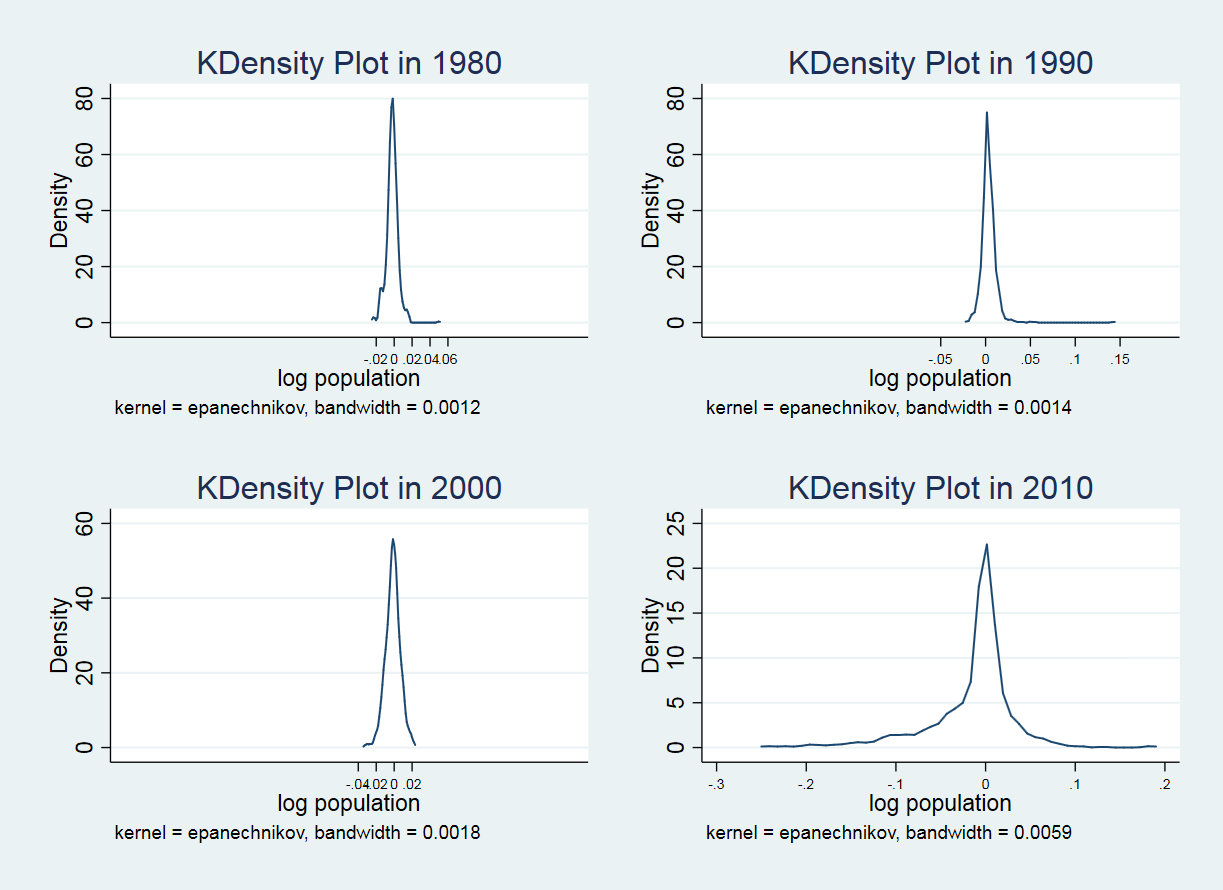
\includegraphics[width=1\textwidth]{KDtotpop_all.png}
\end{figure}



\section{Extension}
\noindent
This section provides an extension of the paper by taking city size into account. Large cities, with its thick labor market, act as a role of "sponge" to mitigate the import competition. Displaced workers can find jobs in larger cities without the need to migrate. This provides the motivation for my extension exercise.
\newline
\newline
To conduct this extension, I start with dividing my sample into two groups: large commuting zones and small commuting zones. The size of commuting zone I use is the commuting zone size in 1990, which is before the China shock kicked in. I include all the control variables, same as the preferred specification from the paper.
\newline
\newline
Table 8 shows the result of whole sample, small commuting zones subsample, and large commuting zone subsample. Two age groups are examined: 15-64 working population and 15-34 young labor force. There is little evidence that NTR Gap has different effect on large and small commuting zones. 
\newline
\newline
To estimate this idea more precisely, I introduce an interaction term to estimate how the effect of NTR Gap changes with size of commuting zone.
\newline
\begin{equation}
\begin{split}
ln(population_{ct}) = & \beta_0 + \beta_1 NTR Gap_c * Post2001_t + \beta _2 X_c * Post2001_t  \\
    & + \beta _3 \Delta ln(population_{c,t-10}) + \beta _4 CZsize_{1990} \\
    & + \beta _5 NTR Gap_c * Post2001_t * CZsize_{1990} + \delta _{rt} + \epsilon _{ct}
\end{split}
\end{equation}
\newline
\newline
\noindent
Table 9 shows the result for this interaction model. For population aged 15-64, bigger cities react less to NTR Gap, as the interaction term is positive and significant at $1\%$ level. For population aged 15-34, the interaction term estimate becomes smaller and not significant, while remains positive. I argue that commuting zone size might be an important factor to consider because displaced workers might be less likely to move if the market is thick.
\newline
\newline

\begin{table}[htbp]\centering
\def\sym#1{\ifmmode^{#1}\else\(^{#1}\)\fi}
\caption{Log CZ Population Changes (Whole Sample, Large, Small CZs)}
\begin{tabular}{l*{6}{c}}
\hline
\hline
\toprule
&\multicolumn{1}{c}{(1)}&\multicolumn{1}{c}{(2)}&\multicolumn{1}{c}{(3)}&\multicolumn{1}{c}{(4)}&\multicolumn{1}{c}{(5)}&\multicolumn{1}{c}{(6)}\\
&\multicolumn{1}{c}{$\Delta ln(pop_{15-64})$}&\multicolumn{1}{c}{Large CZs}&\multicolumn{1}{c}{Small CZs}&\multicolumn{1}{c}{$\Delta ln(pop_{15-34})$}&\multicolumn{1}{c}{Large CZs}&\multicolumn{1}{c}{Small CZs}\\
\hline
\midrule
NTR Gap             &   -0.264** &   -0.263** &   -0.248** &   -0.503***&   -0.505***&   -0.494***\\
                    &  (0.114)   &  (0.115)   &  (0.112)   &  (0.170)   &  (0.168)   &  (0.159)   \\
\addlinespace
Lag    &    0.529***&    0.530***&    0.569***&            &            &            \\
                    &  (0.034)   &  (0.037)   &  (0.044)   &            &            &            \\
\addlinespace
Lag    &            &            &            &    0.338***&    0.324***&    0.344***\\
                    &            &            &            &  (0.047)   &  (0.052)   &  (0.050)   \\
\midrule
Obs        &     1322   &      961   &      961   &     1322   &      961   &      961   \\
\(R^{2}\)           &    0.743   &    0.758   &    0.768   &    0.653   &    0.669   &    0.637   \\
RY FE      &        Y   &        Y   &        Y   &        Y   &        Y   &        Y   \\
\bottomrule
\hline
\multicolumn{7}{l}{\footnotesize Standard errors in parentheses}\\
\multicolumn{7}{l}{\footnotesize * p<.1, ** p<0.05, *** p<0.01}\\
\end{tabular}
\end{table}


\begin{table}[htbp]\centering
\def\sym#1{\ifmmode^{#1}\else\(^{#1}\)\fi}
\caption{Interation Model Estimates}
\begin{tabular}{l*{4}{c}}
\toprule
\hline
\hline 
&\multicolumn{1}{c}{(1)}&\multicolumn{1}{c}{(2)}&\multicolumn{1}{c}{(3)}&\multicolumn{1}{c}{(4)}\\
&\multicolumn{1}{c}{$\Delta ln(pop_{15-64})$}&\multicolumn{1}{c}{}&\multicolumn{1}{c}{$\Delta ln(pop_{15-34})$}&\multicolumn{1}{c}{}\\
\hline 
\midrule
NTR Gap             &   -3.343***&   -2.147***&   -2.557***&   -1.398*  \\
                    &  (0.712)   &  (0.568)   &  (0.969)   &  (0.750)   \\
\addlinespace
Lag 15-64 Change    &    0.591***&    0.563***&            &            \\
                    &  (0.029)   &  (0.032)   &            &            \\
\addlinespace
lpop90             &   -0.007** &   -0.007*  &   -0.004   &   -0.003   \\
                    &  (0.003)   &  (0.003)   &  (0.004)   &  (0.005)   \\
\addlinespace
NTR * lpop90            &    0.244***&    0.146***&    0.151** &    0.070   \\
                    &  (0.056)   &  (0.047)   &  (0.075)   &  (0.060)   \\
\addlinespace
Lag 15-34 Change    &            &            &    0.385***&    0.352***\\
                    &            &            &  (0.044)   &  (0.045)   \\
Controls      &        No  &        Yes   &        No   &        Yes   \\
\midrule
Observations        &     1444   &     1322   &     1444   &     1322   \\
\(R^{2}\)           &    0.730   &    0.750   &    0.625   &    0.654   \\
\hline
\bottomrule
\multicolumn{5}{l}{\footnotesize Standard errors in parentheses}\\
\multicolumn{5}{l}{\footnotesize * p<.1, ** p<0.05, *** p<0.01}\\
\end{tabular}
\end{table}



\section{Conclusion}
\noindent
This paper replicates the main result of "Import Competition and Internal Migration"\cite{greenland2019import}, authored by Greenland, Andrew, John Lopresti, and Peter McHenry and published on \textit{Review of Economics and Statistics} in 2019. The replication result is very close to the original work while slight downward estimates are observed. This paper also has an extension which commuting zone size is taken into account. It is shown that for larger cities, the negative effect of import competition on population growth will be smaller.  

\clearpage 
\bibliographystyle{bibft}\it
\bibliography{bibfile}


\end{document}



